    % Tasks:
% Put in estimate of galactic NH (Moritz)
% Dickey and Lockman, 1990, Annu. Rev. Astron. Astrophys., 28, 215
% get: 1.73 e20 - maybe plot second model with nh fixed? - plot done, but not yet included
% Get TESS lightcurve to check for variability (MMax) - done
% Is a jet reasonable (eqn 6) (Moritz to put some numbers in)
% Arcus simulations (Moritz)
% Check if X-East and X-West coincide with GAIA sources (i.e. they are foreground stars) - good hint from Christian (Moritz) - done. No GAIA DR2 or 2MASS sources are close to X-East and X-North.
% Consolidate discussion on shock physics - mostly done
% discuss variability and magnetic field
% plot of L_X / L_bol for some classes of objects. What's the other axis? rosby number? Age? Period? - done (Fig. 5)



%% using aastex version 6.3
\documentclass[linenumbers]{aastex631}
\usepackage{amsmath}
\usepackage{amssymb}

\newcommand{\be}{\begin{equation}}
\newcommand{\ee}{\end{equation}}

%% The default is a single spaced, 10 point font, single spaced article.
%% There are 5 other style options available via an optional argument. They
%% can be invoked like this:
%%
%% \documentclass[arguments]{aastex631}
%%
%% where the layout options are:
%%
%%  twocolumn   : two text columns, 10 point font, single spaced article.
%%                This is the most compact and represent the final published
%%                derived PDF copy of the accepted manuscript from the publisher
%%  manuscript  : one text column, 12 point font, double spaced article.
%%  preprint    : one text column, 12 point font, single spaced article.
%%  preprint2   : two text columns, 12 point font, single spaced article.
%%  modern      : a stylish, single text column, 12 point font, article with
%% 		  wider left and right margins. This uses the Daniel
%% 		  Foreman-Mackey and David Hogg design.
%%  RNAAS       : Supresses an abstract. Originally for RNAAS manuscripts
%%                but now that abstracts are required this is obsolete for
%%                AAS Journals. Authors might need it for other reasons. DO NOT
%%                use \begin{abstract} and \end{abstract} with this style.
%%
%% Note that you can submit to the AAS Journals in any of these 6 styles.
%%
%% There are other optional arguments one can invoke to allow other stylistic
%% actions. The available options are:
%%
%%   astrosymb    : Loads Astrosymb font and define \astrocommands.
%%   tighten      : Makes baselineskip slightly smaller, only works with
%%                  the twocolumn substyle.
%%   times        : uses times font instead of the default
%%   linenumbers  : turn on lineno package.
%%   trackchanges : required to see the revision mark up and print its output
%%   longauthor   : Do not use the more compressed footnote style (default) for
%%                  the author/collaboration/affiliations. Instead print all
%%                  affiliation information after each name. Creates a much
%%                  longer author list but may be desirable for short
%%                  author papers.
%% twocolappendix : make 2 column appendix.
%%   anonymous    : Do not show the authors, affiliations and acknowledgments
%%                  for dual anonymous review.
%%
%% these can be used in any combination, e.g.
%%
%% \documentclass[twocolumn,linenumbers,trackchanges]{aastex631}
%%
%% AASTeX v6.* now includes \hyperref support. While we have built in specific
%% defaults into the classfile you can manually override them with the
%% \hypersetup command. For example,
%%
%% \hypersetup{linkcolor=red,citecolor=green,filecolor=cyan,urlcolor=magenta}
%%
%% will change the color of the internal links to red, the links to the
%% bibliography to green, the file links to cyan, and the external links to
%% magenta. Additional information on \hyperref options can be found here:
%% https://www.tug.org/applications/hyperref/manual.html#x1-40003
%%
%% Note that in v6.3 "bookmarks" has been changed to "true" in hyperref
%% to improve the accessibility of the compiled pdf file.
%%
%% If you want to create your own macros, you can do so
%% using \newcommand. Your macros should appear before
%% the \begin{document} command.
%%

%% Reintroduced the \received and \accepted commands from AASTeX v5.2
%\received{March 1, 2021}
%\revised{April 1, 2021}
%\accepted{\today}

%% Command to document which AAS Journal the manuscript was submitted to.
%% Adds "Submitted to " the argument.
%\submitjournal{PSJ}

%%
%% For manuscript without any need to use \collaboration the
%% \AuthorCollaborationLimit command from v6.2 can still be used to
%% show a subset of authors.
%
%\AuthorCollaborationLimit=2
%
%% will only show Schwarz & Muench on the front page of the manuscript
%% (assuming the \collaboration and \nocollaboration commands are
%% commented out).
%%
%% Note that all of the author will be shown in the published article.
%% This feature is meant to be used prior to acceptance to make the
%% front end of a long author article more manageable. Please do not use
%% this functionality for manuscripts with less than 20 authors. Conversely,
%% please do use this when the number of authors exceeds 40.
%%
%% Use \allauthors at the manuscript end to show the full author list.
%% This command should only be used with \AuthorCollaborationLimit is used.

%% The following command can be used to set the latex table counters.  It
%% is needed in this document because it uses a mix of latex tabular and
%% AASTeX deluxetables.  In general it should not be needed.
%\setcounter{table}{1}

%%%%%%%%%%%%%%%%%%%%%%%%%%%%%%%%%%%%%%%%%%%%%%%%%%%%%%%%%%%%%%%%%%%%%%%%%%%%%%%%
%%
%% The following section outlines numerous optional output that
%% can be displayed in the front matter or as running meta-data.
%%
%% If you wish, you may supply running head information, although
%% this information may be modified by the editorial offices.
\shorttitle{X-ray emission from TYC 2597-735-1}
\shortauthors{G\"unther et al.}

\graphicspath{{./}{figures/}}
%% This is the end of the preamble.  Indicate the beginning of the
%% manuscript itself with \begin{document}.

\begin{document}

\title{X-ray emission from candidate stellar merger remnant TYC 2597-735-1 and its Blue Ring Nebula}

%% LaTeX will automatically break titles if they run longer than
%% one line. However, you may use \\ to force a line break if
%% you desire. In v6.31 you can include a footnote in the title.

%% A significant change from earlier AASTEX versions is in the structure for
%% calling author and affiliations. The change was necessary to implement
%% auto-indexing of affiliations which prior was a manual process that could
%% easily be tedious in large author manuscripts.
%%
%% The \author command is the same as before except it now takes an optional
%% argument which is the 16 digit ORCID. The syntax is:
%% \author[xxxx-xxxx-xxxx-xxxx]{Author Name}
%%
%% This will hyperlink the author name to the author's ORCID page. Note that
%% during compilation, LaTeX will do some limited checking of the format of
%% the ID to make sure it is valid. If the "orcid-ID.png" image file is
%% present or in the LaTeX pathway, the OrcID icon will appear next to
%% the authors name.
%%
%% Use \affiliation for affiliation information. The old \affil is now aliased
%% to \affiliation. AASTeX v6.31 will automatically index these in the header.
%% When a duplicate is found its index will be the same as its previous entry.
%%
%% Note that \altaffilmark and \altaffiltext have been removed and thus
%% can not be used to document secondary affiliations. If they are used latex
%% will issue a specific error message and quit. Please use multiple
%% \affiliation calls for to document more than one affiliation.
%%
%% The new \altaffiliation can be used to indicate some secondary information
%% such as fellowships. This command produces a non-numeric footnote that is
%% set away from the numeric \affiliation footnotes.  NOTE that if an
%% \altaffiliation command is used it must come BEFORE the \affiliation call,
%% right after the \author command, in order to place the footnotes in
%% the proper location.
%%
%% Use \email to set provide email addresses. Each \email will appear on its
%% own line so you can put multiple email address in one \email call. A new
%% \correspondingauthor command is available in V6.31 to identify the
%% corresponding author of the manuscript. It is the author's responsibility
%% to make sure this name is also in the author list.
%%
%% While authors can be grouped inside the same \author and \affiliation
%% commands it is better to have a single author for each. This allows for
%% one to exploit all the new benefits and should make book-keeping easier.
%%
%% If done correctly the peer review system will be able to
%% automatically put the author and affiliation information from the manuscript
%% and save the corresponding author the trouble of entering it by hand.


\author[0000-0003-4243-2840]{Hans Moritz G{\"u}nther}
\affiliation{MIT Kavli Institute for Astrophysics and Space Research, 77 Massachusetts Avenue, Cambridge, MA 02139, USA}
\author[0000-0002-8636-3309]{Keri Hoadley}
\affiliation{The University of Iowa, Dept. of Physics \& Astronomy, Van Allen Hall, Iowa City, IA, 52242, USA}
\affiliation{California Institute of Technology, Dept. of Physics, Mathematics, and Astronomy, Cahill Center for Astronomy \& Astrophysics, Pasadena, CA 91125, USA}
\author[0000-0002-3164-9086]{Maximilian N. G{\"u}nther}
\thanks{Juan Carlos Torres Fellow, ESA Research Fellow}
\affiliation{Department of Physics, and Kavli Institute for Astrophysics and Space Research, Massachusetts Institute of Technology, 77 Massachusetts Avenue, Cambridge, MA 02139, US}
\affiliation{European Space Agency (ESA), European Space Research and Technology Centre (ESTEC), Keplerlaan 1, 2201 AZ Noordwijk, The Netherlands}
\author[0000-0002-4670-7509]{Brian D. Metzger}
\affiliation{Department of Physics and Columbia Astrophysics Laboratory, Columbia University, Pupin Hall, New York, NY 10027, USA}
\affiliation{Center for Computational Astrophysics, Flatiron Institute, 162 5th Ave, New York, NY 10010, USA}
\author[0000-0002-5094-2245]{P. C. Schneider}
\affiliation{Hamburger Sternwarte, Gojenbergsweg 112, 21029 Hamburg, Germany}
\author[0000-0002-9632-6106]{Ken J. Shen}
\affiliation{Department of Astronomy and Theoretical Astrophysics Center, University of California, Berkeley, CA 94720, USA}



%% Note that the \and command from previous versions of AASTeX is now
%% depreciated in this version as it is no longer necessary. AASTeX
%% automatically takes care of all commas and "and"s between authors names.

%% AASTeX 6.31 has the new \collaboration and \nocollaboration commands to
%% provide the collaboration status of a group of authors. These commands
%% can be used either before or after the list of corresponding authors. The
%% argument for \collaboration is the collaboration identifier. Authors are
%% encouraged to surround collaboration identifiers with ()s. The
%% \nocollaboration command takes no argument and exists to indicate that
%% the nearby authors are not part of surrounding collaborations.

%% Mark off the abstract in the ``abstract'' environment.
\begin{abstract}
Tight binary or multiple star systems can interact through mass transfer and follow vastly different evolutionary pathways than single stars. The star TYC 2597-735-1 is a candidate for a recent stellar merger remnant resulting from a coalescence of a low-mass companion with a primary star a few thousand years ago. This violent event is evident in a conical outflow (``Blue Ring Nebula'') emitting in UV light and surrounded by leading shock filaments observed in H$\alpha$ and UV emission. From Chandra data, we report the detection of X-ray emission from the location of TYC 2597-735-1 with a luminosity $\log(L_\mathrm{X}/L_\mathrm{bol})=-5.3$.  A TESS lightcurve confirms a period of about 14~days. Together, this indicates ongoing stellar activity and the presence of strong magnetic fields on TYC 2597-735-1. Supported by stellar evolution models of merger remnants, we interpret the stellar activity as dynamo action associated with a newly formed convection zone in the atmosphere of TYC 2597-735-1, though internal shocks at the base of an accretion-powered jet cannot be ruled out.  We speculate that this object will evolve into an FK Com type source, i.e.\ a class of rapidly spinning magnetically active stars for which a merger origin has been proposed but for which no relic accretion or large-scale nebula remains visible.  We also detect X-ray emission from two small regions close to the outer shock fronts in the Blue Ring Nebula, which may arise from either inhomogenities in the circumstellar medium or in the mass and velocity distribution in the merger-driven outflow.

\end{abstract}

%% Keywords should appear after the \end{abstract} command.
%% The AAS Journals now uses Unified Astronomy Thesaurus concepts:
%% https://astrothesaurus.org
%% You will be asked to selected these concepts during the submission process
%% but this old "keyword" functionality is maintained in case authors want
%% to include these concepts in their preprints.
\keywords{}


\section{Introduction} \label{sec:intro}
%%%% New intro: Outline
%% 1. TYC and BRN discovery as recent (1000's years old) stellar merger event
%% 2. Prime laboratory to test and explore theorized behaviors and evolution of such systems
%% 3. Serendipitous discovery of X-ray emission by Chandra begs the question: what is generating this high energy radiation both in the BRN and near TYC?
%% 4. Outline of study
Binary and multi-star systems make up over 1/3 of the star systems in the Galaxy \citep{Raghavan+2010}. It is no surprise, then, that closely orbiting binary stars will commonly interact through events that exchange and shed matter from one star to another (e.g., common envelope evolution (CEE)) or end with the complete engulfment of one star by another (e.g., \citealt{Ivanova+2013}). TYC 2597-735-1 is one of only a few examples of a recent ($t \sim$ 2,000 - 5,000 years ago), unobscured (E(B-V) $\sim$ 0.02) stellar merger remnant found to date \citep{2020Natur.587..387H}.
Other examples include \object{BP Psc} \citep{Zuckerman_2008}, \object{TYC 4144 329 2} \citep{Melis_2009}, and FK~Com type stars \citep[see, e.g.,][for a very detailed study of FK Com itself]{2016ApJS..223....5A}.
This makes TYC 2597-735-1 a rare astrophysical laboratory to test models for the physical processes by which stars merge and for the long-term evolution of the stellar remnants left over from such mergers.

One key stellar behavioral shift that may arise as a result of a stellar merger is the generation of a strong magnetic field \citep{Schneider+2016}. Roughly 10\% of intermediate- to high-mass stars ($M_{\star} \gtrsim$ 1.5 $M_{\odot}$) possess strong magnetic fields, whose origins are currently unknown (e.g., \citealt{Donati+2009,Fossati+2015,Grunhut+2017}). \citet{Soker&Tylenda2007} showed that the extended envelope of a merger product may host a large convective region. Paired with a rapid rotation rate that also arises from the merger process, an efficient dynamo may result, giving rise to strong magnetic activity. The presence of magnetic fields has strong implications on the long-term evolution of the stellar merger system. For example, magnetic fields may drive magnetorotational accretion of surrounding material, help slow down rapidly rotating stars via magnetic braking, and power jets (e.g., \citealt{Schneider+2020}). All these mechanisms, over long timescales, have consequences on the final outcome of a stellar merger remnant as it settles to its equilibrium state.

\citet{Soker&Tylenda2007} suggest the strongest magnetic activity tied to a stellar merger's revitalized dynamo may last centuries. Many other recent suspected stellar mergers like red luminous novae are obscured from view by outflows ejected during the merger event itself (e.g., \citealt{Bond+2003, Tylenda+2016}). TYC 2597-735-1 shows evidence that it harbors a persisting, strong magnetic field \citep[e.g., H$\alpha$ emission and variability, radial velocity shifts strongly correlated with the Ca II IRT stellar atmospheric features,][]{2020Natur.587..387H}. One way to test whether its hypothetical magnetic field exists is to look for signs of X-ray emission at TYC 2597-735-1 and compare its luminosity to the remnant's bolometric luminosity \citep{Soker&Tylenda2007}.

TYC 2597-735-1 and the last vestiges of its dissolving outflow, the ``Blue Ring Nebula'' (BRN; \citealt{2020Natur.587..387H}), were partially observed by chance with Chandra over a decade ago. Here, we report the findings of this serendipitous \emph{Chandra} observation and present a new \emph{TESS} lightcurve. We explore whether the X-ray emission observed at TYC 2597-735-1 is consistent with dynamo-driven magnetic field activity or other sources near the star. We summarize the stellar properties of TYC 2597-735-1 in Section~\ref{sec:properties}. In Section~\ref{sec:data}, we describe the observations, the source detection methods implemented to retrieve X-ray signal from regions in the BRN and around TYC 2597-735-1 and the X-ray properties of these regions. In Section~\ref{sec:discussion}, we explore different physical mechanisms that may explain the X-ray luminosity and spectral characteristics observed for TYC 2597-735-1 and place physical limits on the properties of the BRN shock region from its X-ray diagnostics. We conclude in Section~\ref{sec:summary} with a summary.

\section{Properties of TYC 2597-735-1}
\label{sec:properties}

\begin{table}
\caption{\textbf{Present day} stellar properties from \citet{2020Natur.587..387H} \label{tab:parameters}}
\begin{tabular}{lcr}
\hline \hline
parameter & symbol & value \\
\hline
distance & $d$ & $1.9 \pm 0.1$ kpc\\
luminosity & $L_\mathrm{bol}$ & $110 \;L_\sun{}$\\
radius & $R_*$ & $11\;R_\sun{}$\\
mass & $M_*$ & $1-2.1\;M_\sun{}$\\
temperature & $T_\mathrm{eff}$ & 5850 K\\
surface gravity & $g$ & 600 cm s$^{-2}$\\
rotational broadening & $v \sin i$ & 6.5 km s$^{-1}$\\
accretion rate & $\dot M_\mathrm{acc}$ & $<1.5 \times 10^{-7}\; M_\sun{}\;\mathrm{yr}^{-1}$\\
RV period & $P_\mathrm{RV}$ & 13.7 days \\
time since merger & & 1000-5000 yr\\
\hline
\end{tabular}
\end{table}

\cite{2020Natur.587..387H} present imaging and spectroscopic information for TYC 2597-735-1 and derive stellar properties, which we summarize in Table~\ref{tab:parameters}. They detect several signs of stellar activity, including variable H$\alpha$ emission line profiles and radial-velocity (RV)  variations with a period around 13.7~days. \cite{2020Natur.587..387H} argue that line profiles and the parameter space for a potential companion favor an interpretation of the RV data as caused by stellar activity, potentially in the polar regions.

\cite{2020Natur.587..387H} interpret the combination of the bright BRN and the unusual stellar parameters in a stellar merger scenario, where a low-mass ($0.1\;\mathrm{M}_\sun$), short-period companion merged with the primary star a few thousand years ago. In the process of that merger, a circumstellar disk with an inner radius of 0.1~au was formed. Today, material from that disk is accreting onto the central star. The merger also caused the ejection of a conical outflow moving at velocities of around 400~km~s$^{-1}$. Our line-of-sight is close to the axis of the outflow and we see the approaching and receding flows projected onto the sky as the rings of the BRN.
The BRN is seen brightly in the UV as a diffuse ring and, at further distance from TYC 2597-735-1, narrow H$\alpha$ filaments (Figure~\ref{fig:chandraimage}). \cite{2020Natur.587..387H} explain the H$\alpha$ as the forward shock of the outflow, caused by the ejecta driving a shock wave into the circumstellar medium or ISM, while the UV emission should be dominated by molecular H$_2$ emission that is excited by a reverse shock. This reverse shock is caused by the deceleration of the outflow with the circumstellar medium/ISM and now travels backwards through the outflow.

\section{Data analysis} \label{sec:data}
\subsection{Chandra data reduction}
TYC 2597-735-1 was observed by Chandra on 2007-11-26 for 8.7~ks.
We retrieved Chandra OBSID 8636 from  the archive and reprocessed it with CIAO 4.13.0 \citep{2006SPIE.6270E..1VF} in the VFAINT mode, which reduces the background compared to the default FAINT mode processing. This is a serendipitous observation where TYC 2597-735-1 falls by chance on one of the outer CCDs (CCD S2 on the ACIS-S array). TYC 2597-735-1 is located close to the chip edge and only a fraction of the H$\alpha$ and UV emitting regions around the central star is covered in the observations. Because TYC 2597-735-1 is located off-axis, the PSF is significantly wider than on-axis. Figure~\ref{fig:chandraimage} shows the positions of individual X-ray photons overlayed on the H$\alpha$ images and UV emission contours from \citet{2020Natur.587..387H}, limited to a soft X-ray band.
\begin{figure*}
    \centering
    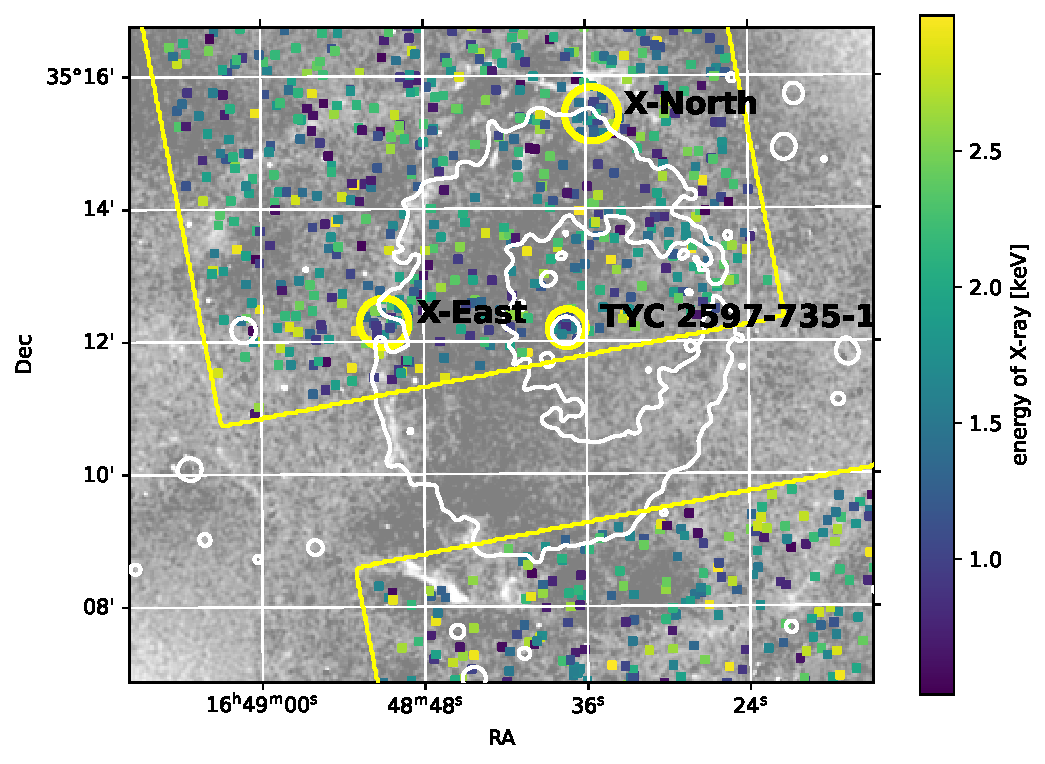
\includegraphics[width=\textwidth]{figures/chandraimage.pdf}
\caption{X-ray emission around TYC 2597-735-1. The grey-scale image shows H$\alpha$ emission and the white contours outline the UV emission. Data for both is taken from \citet{2020Natur.587..387H}, see there for details. \textbf{The white contour line is drawn at} $6\times 10^{-4}$~counts~s$^{-1}$~pix$^{-1}$ \textbf{in an image smoothed by a Gaussian filter with} $\sigma=4.5$\arcsec{} \textbf{(3 pixels). This level corresponds to twice the background rate, and is} $>10\sigma$ \textbf{significant in the smoothed image.}
    The colored squares mark the position of individual X-ray photons, where the color denotes the energy of each particular photon. Only photons in the energy range given on the color bar are shown. Yellow circles mark the position of the three detected sources and their 90\% PSF size, which we use as the extraction region to extract spectra. The thin yellow lines outlines the area covered by Chandra in the observation.}
    \label{fig:chandraimage}
\end{figure*}

\subsection{X-ray source detection}
\label{sec:xraydetection}
We expect any emission from the outflows to be soft (section~\ref{sec:outflow}), but somewhat absorbed due to the large distance of TYC 2597-735-1. To reduce the high-energy background, which can overwhelm weak, soft sources, we construct a narrow band image in the 1-2~keV range
and run a source detection with the CIAO \texttt{wavdetect} task, which convolves the input image with a wavelet, taking the size of the PSF at that image location into account. We bin up the image such that it contains $2.6\times10^4$ pixels in the region of interest (the bottom half of the CCD that contains TYC 2597-735-1, marked by the yellow outline in Figure~\ref{fig:chandraimage}) and set the significance threshold such that we expect 0.25 false positive sources in this region. That way, any source detected by \texttt{wavdetect} is likely to be real. We find three sources (table~\ref{tab:src}), all of which coincide with UV/optical emission features. All three sources have similar count rates and similar PSF sizes and thus similar positional uncertainties of about 2\arcsec{}.

\begin{table*}
\caption{Detected X-ray sources in the 0.5-2.0~keV band\label{tab:src}}
\begin{tabular}{ccccccc}
\hline \hline
name & RA & DEC & $\sigma_\mathrm{RA}$ & $\sigma_\mathrm{DEC}$ & NET COUNTS & BKG COUNTS\\
 &  &  & $\mathrm{{}^{\prime\prime}}$ & $\mathrm{{}^{\prime\prime}}$ & $\mathrm{ct}$ & $\mathrm{ct}$ & $\mathrm{ct}$ & $\mathrm{ct}$ \\
\hline
TYC 2597-735-1 & $16^{\mathrm{h}}48^{\mathrm{m}}38^{\mathrm{s}}$ & $35^\circ12{}^\prime12{}^{\prime\prime}$ & 3.1 & 2.0 & $9.8 \pm 3.6$ & $3.17 \pm 0.02$ \\
X-North & $16^{\mathrm{h}}48^{\mathrm{m}}35^{\mathrm{s}}$ & $35^\circ15{}^\prime31{}^{\prime\prime}$ & 2.6 & 3.3 & $7.1 \pm 3.3$ & $3.91 \pm 0.02$\\
X-East & $16^{\mathrm{h}}48^{\mathrm{m}}50^{\mathrm{s}}$ & $35^\circ12{}^\prime19{}^{\prime\prime}$ & 4.1 & 1.7 & $15.5 \pm 4.7$ & $6.47 \pm 0.03$ \\
\hline
\end{tabular}
\end{table*}



We detect a source at the location of TYC 2597-735-1 with (in our narrow band image) $9\pm3$ counts on a background of $1.52\pm0.01$ counts. The background is known to a high precision because \texttt{wavdetect} determines it over a large area. Additionally, the probability that any one source randomly overlaps with the known position of TYC 2597-735-1 within the 90\% PSF radius (0.28 arcmin for an energy of 1.5~keV and at the position of TYC 2597-735-1) is only 0.2\%. Thus, we regard this as a highly reliable detection of X-ray emission from TYC 2597-735-1, albeit with large uncertainties on flux and spectral properties due to the small number of counts.

We do detect two other features that are both located just inside the ring of H$\alpha$. One of them is almost due North of TYC 2597-735-1, and the other one to the East (Fig.~\ref{fig:chandraimage}, see table~\ref{tab:src} for source properties).  Neither the GAIA DR2 \citep{2016A&A...595A...1G,2018A&A...616A...1G} nor the 2MASS \citep{2006AJ....131.1163S} catalogs show any point sources coinciding with these features; thus the X-ray emission cannot be caused by a foreground star. Together with the soft X-ray spectrum (see below) this also rules out most classes of X-ray background objects. Again, the fact that both features are located at a physically meaningful position between forward and the reverse shock of the BRN (seen as H$\alpha$ and the UV emission shown in Fig.~\ref{fig:chandraimage}) argues that these are not background fluctuations, but probably very weak sources that are physically associated with the outflow. However, the number of detected photons is low and only deeper X-ray observations will be able to unambiguously confirm these detections.
All three sources are compatible with point sources. While we expect that the latter two sources are spatially extended, since the H$\alpha$ and the UV emission in the region is also extended, the low count number does not allow us to actually fit the source shape or extent, so we treat them like point sources below.

We also search for extended emission on larger scales that coincide with either the reverse shock where the the FUV emission is seen (using a region bounded by the white contours  in Fig.~\ref{fig:chandraimage}) or in the space between forward and reverse shock, i.e.\ in a ring on the outside of the white contour in Fig.~\ref{fig:chandraimage} that contains the sources labelled ``X-North'' and ``X-East''. However, we do not know a priori which level of contour lines might be correlated, so the selection of the region is somewhat arbitrary. We do not see significantly enhanced emission --except for the three point-like sources discussed above-- compared to a background region on the northern half of the chip. To obtain an order-of-magnitude estimate how bright an extended source would have to be for a secure detection, we take the $3\sigma$ uncertainty of the observed background flux (about $10^{-5}$~counts~s$^{-1}$~arcsec$^{-2}$) in the same 1-2~keV energy range as for the source detection above and convert that the number into an energy flux per surface area in the plane of the sky. We find that emission would have to be stronger than a few times $10^{31}$~erg~s$^{-1}$~pc$^{-2}$ in this band to be detected significantly above the background.

\subsection{X-ray source properties}
\label{sec:xrayspectra}
For all three regions, the detected soft photons are well distributed over the observing time; we do not see strong clustering that would indicate a large flare, but given the low count numbers, variability with factors of a few cannot be excluded.

We extract spectra for all three sources using circular extraction regions that encompass 90\% of the PSF at 1.5~keV at the location of the source. A background spectrum is extracted from a large region on the same chip located outside of the UV contours shown in Fig~\ref{fig:chandraimage}. Below 7~keV, the background is well described by a flat component, except for a significant feature around 2.2~keV \citep[caused by fluorescence of gold in the instrument,][]{2021arXiv210811234S}. Therefore, we exclude the regions 2.0-2.5~keV and $>7.0$~keV from fitting. We then simultaneously fit the source and background spectra using a modified Cash statistic \citep{1979ApJ...228..939C} as implemented in Sherpa \citep{2007ASPC..376..543D,doug_burke_2021_4428938}. To fit source emission, we use a model of an absorbed, collisionally-excited plasma \citep[APEC model,][]{2012ApJ...756..128F} and add the flat background model, scaled for the different extraction regions. That way, we avoid subtracting the background and retain Poisson statistics. All fits are done on unbinned data, but the spectra are shown binned for display in Figs.~\ref{fig:TYC_spec} and \ref{fig:combined}.

The spectrum for TYC 2597-735-1 is shown in Fig.~\ref{fig:TYC_spec}. We fit $N_\mathrm{H}=(6\pm5)\times10^{21}$~cm$^{-2}$ and a plasma temperature in the range 0.1-1.5~keV, where the low end of the temperature range requires very large values of $N_\mathrm{H}$ and emission measure. For temperatures around 1~keV, common for stellar sources, the unabsorbed flux is of order $10^{-13}$~erg~s$^{-1}$~cm$^{-2}$, which corresponds to $3\times 10^{30}$~erg~s$^{-1}$ with uncertainties of a factor of a few.

The total galactic absorption in this line of sight is about $N_\mathrm{H}=2\times10^{21}$~cm$^{-2}$ \citep{1990ARA&A..28..215D}. Fitting just the temperature, but fixing the absorbing column density leads to a model with similar spectral shape (\textbf{green} line in Fig.~\ref{fig:TYC_spec}), but a preferred higher temperature $kT=4_{-3}^{+\infty}$~keV.
For low count numbers, there is a fundamental degeneracy between plasma temperature and absorbing column density: A cool, but bright plasma with a high $N_\mathrm{H}$ produces a spectrum very similar to the spectrum emitted from a hotter, but less absorbed plasma.
Assuming the hotter spectrum, a weaker source ($2\times10^{-14}$~erg~s$^{-1}$~cm$^{-2}$, which corresponds to $5\times 10^{29}$~erg~s$^{-1}$) could be sufficient to explain the observed photons; on the other hand, there could still be a second, cooler, component that is hidden by the $N_\mathrm{H}$, thus the flux given is a lower limit only. \cite{2020Natur.587..387H} found essentially no reddening towards TYC 2597-735-1, but depending on the position of the X-ray emitting gas it is possible that accretion columns or the disk are in our line-of-sight and that the $N_\mathrm{H}$ observed in X-rays is larger than the reddening of the optical spectra.

\begin{figure}
    \plotone{figures/TYC_spec.pdf}
    \caption{Spectrum of TYC 2597-735-1 binned to two counts per bin for display purposes. Error bars are shown just to guide the eye. The orange line shows the best fit model with $N_\mathrm{H}$ as a fitted parameter, for the green model $N_\mathrm{H}$ is fixed as described in the text. Black crosses show the background rate, scaled from a much larger area. The background feature that caused us to ignore the region 2.0-2.5~keV (grey) in the fit is also visible. Error bars on the background are omitted for clarity.
    \label{fig:TYC_spec}}
\end{figure}

We combined the spectra for X-East and X-North because the count number is very low and X-ray properties (see the color of the detected photons in Fig.~\ref{fig:chandraimage}) and location (between H$\alpha$ ring and UV emission) are similar.
We fit $N_\mathrm{H}=(1.3_{-0.6}^{+2})\times10^{22}$~cm$^{-2}$ and a plasma temperature of $0.5_{-0.3}^{+\infty}$~keV (Fig.~\ref{fig:combined}). For temperatures around 0.5~keV, which we will argue are physically reasonable in Sect~\ref{sec:outflow}, the unabsorbed flux is of order $3 \times 10^{-13}$~erg~s$^{-1}$~cm$^{-2}$, which corresponds to $10^{31}$~erg~s$^{-1}$ with uncertainties of a factor a few. As in the case for TYC 2597-735-1, a hotter source with a lower flux seen through a lower absorbing column density could also generate the observed spectrum.
\begin{figure}
    \plotone{figures/combined.pdf}
    \caption{Combined spectrum from the two X-ray detected regions in the outflow. See Fig.~\ref{fig:TYC_spec} for an explanation of symbols.
    \label{fig:combined}}
\end{figure}


\subsection{Optical photometry}
\label{sec:TESS}
The Transiting Exoplanet Survey Satellite (TESS; \citealt{Ricker2015}) observed TYC 2597-735-1 in its sector 25 and camera 1 from 2020-May-13 until 2020-Jun-08.
TESS is an optical photometry mission with four 24x24 degree cameras operating in the 600-1000\,nm range. The spacecraft scans through the entire sky in sectors of $\sim28$\,day duration, whereby each sector is divided into two satellite orbits of $\sim14$\,day duration.
We identify TYC 2597-735-1 as TIC 284856863 in the TESS Input Catalog version 8 \citep{Stassun2019} and find that it fell into TESS's full-frame images with 30 min cadence.
We retrieve the mission's official MIT quick-look-pipeline (QLP) light curve from the High-Level Science Products (HLSP) via the Mikulski Archive for Space Telescopes (MAST) archive.
We also estimate the background flux from the target pixel files (TPFs) via the tools \texttt{tesscut} \citep{Brasseur2019} and \texttt{eleanor} \citep{Feinstein2019}.

Inspecting the detrended light curve and corresponding background flux, we find significant variability (Fig.~\ref{fig:TESS_light_curve}).
This could be due to either intrinsic stellar variability or instrument systematics, or a combination of both.
On the one hand, the radial velocity signal from TYC 2597-735-1 also showed a period of 13.7 days \citep{2020Natur.587..387H}. This would match the period of the two major brightness increases towards the ends of each TESS orbit (TJD 1,990-1,995 and 2,005-2,010; where TJD = $\mathrm{BJD_{TDB}}$ - 2,457,000).

On the other hand, the TESS data release notes\footnote{\url{https://tasoc.dk/docs/release_notes/tess_sector_25_drn36_v02.pdf}} state that Earth's scattered light particularly affected this sector and camera. These notes, along with our inspection of the local background flux (Fig.~\ref{fig:TESS_light_curve}) and the light curves of neighboring stars of similar brightness (not shown here), suggest that these systematics affected mainly the start of each orbit. This means the end of each orbit should remain reliable.

However, the similarity of the expected stellar rotation period and the TESS orbit duration (both $\sim14$\,days) make it difficult to disentangle the true origin of the variability. TESS will re-observe TYC 2597-735-1 in sectors 51 and 52 (from 2022-Apr-22 until 2022-Jun-13). This extended observing window, the possibility of increased observation cadence (2\,min or even 20\,s cadence), and the improved visibility will help to better understand TYC 2597-735-1's behavior at optical wavelengths.

\begin{figure*}
    \centering
    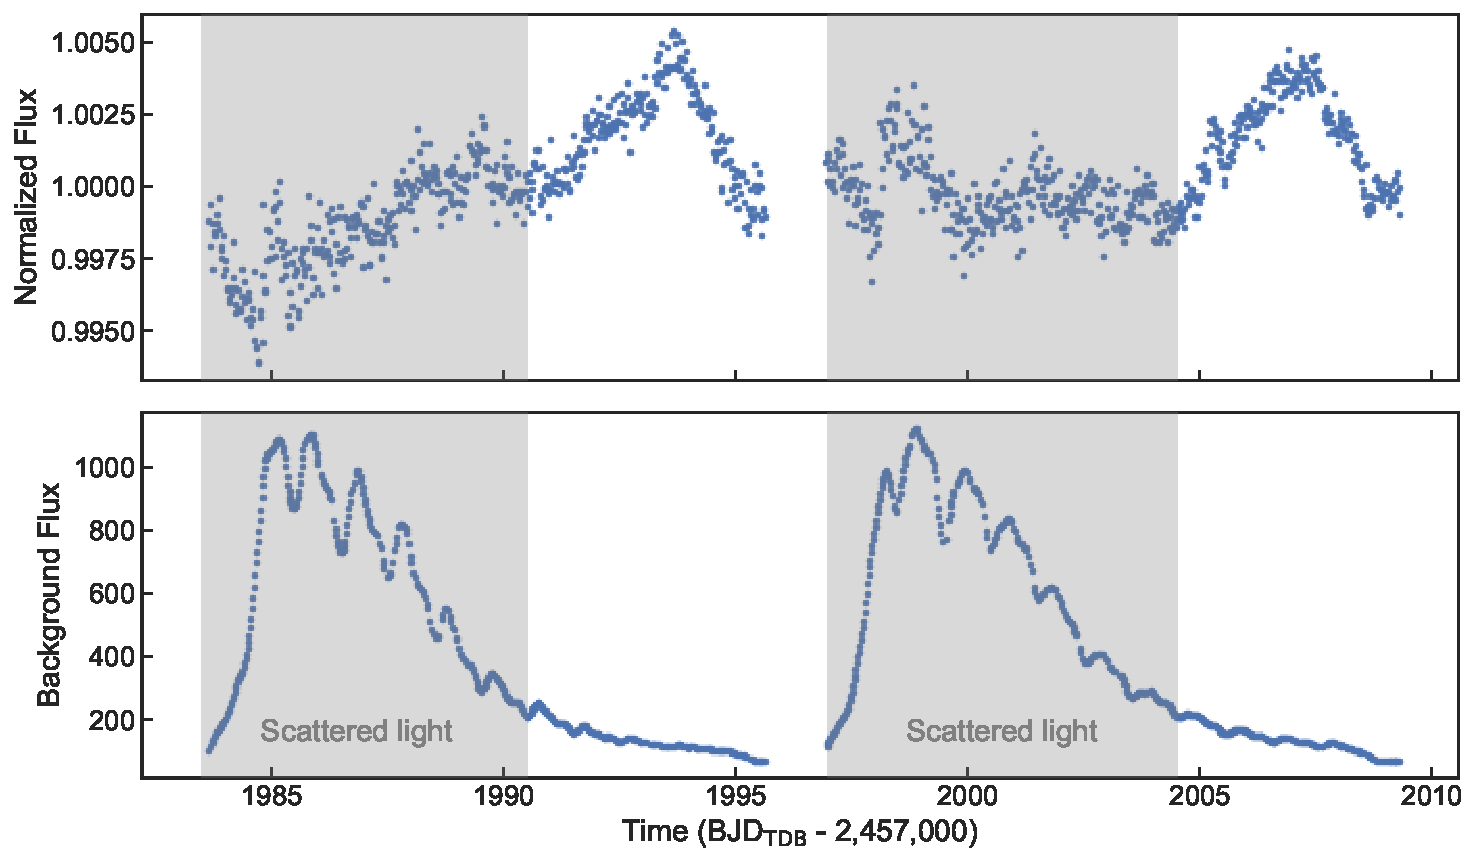
\includegraphics[width=0.8\textwidth]{figures/TESS_light_curve.pdf}
    \caption{TESS light curve and background flux for TYC 2597-735-1. The observations taken in sector 25 with camera 1 range from 2020-May-13 until 2020-Jun-08. The light curve has been corrected for background effects and displays significant variability. While the start of each TESS orbit suffer from systematics caused by Earth's scattered light (grey-shaded areas), the end of each orbit shows brightness increases that could be of astrophysical nature.
    \label{fig:TESS_light_curve}}
\end{figure*}

\cite{2020Natur.587..387H} noticed an RMS scatter around 0.008~mag --significantly larger than the formal uncertainties-- between runs of ground-based $B$ band observations between 2015 and 2019. They attributed this to systematic calibration uncertainties. However, given the variability in the TESS lightcurve on a similar level, this might instead be a signature of stellar rotation.


\section{Discussion}  \label{sec:discussion}
In stellar sources, X-rays mostly originate from optically thin, collisionally excited plasma with temperatures of a few MK. The plasma can be either heated by magnetic reconnection as in the solar corona, or in shocks (accretion shocks or shocks in winds or jets). Unless the density is very low ($<10^5$~cm$^{-3}$ or so), we can assume that the plasma is in an equilibrium ionization state \citep{2007A&A...466.1111G}.
%
%\subsection{X-rays from shocks}
%Shocks convert bulk kinetic energy into thermal energy. Possible scenarios here are an accretion shock where material falls from the disk onto the star with close to free-fall velocity, or shocks in outflows. The latter might be seen in different locations: When the outflow runs into the (almost) stationary ISM (forward-shock), the front of the outflowing material is decelerated, which also causes a reverse shock to pass back through the outflow material. Lastly, changes of the outflow velocity over time can lead to internal working surfaces that travel along the flow as faster material catches up with previous slower ejecta.
Before we discuss possible mechanisms to generate X-ray for TYC 2597-735-1 in Sect.~\ref{sec:discussTYC} and for the resolved outflow in Sect.~\ref{sec:outflow}, we summarize the density and temperatures in strong hydrodynamical shocks, since several possible scenarios involve shock heated plasma.
%Assume material of pre-shock density $n_{\rm pre}$ is moving with velocity $v_{\rm pre}$ into a stationary external medium (the ISM in the case of an outflow termination shock or the stellar photosphere in the case of an accretion shock) of particle density $n_{\rm ext}$.
Assume material of velocity $v_{\rm ej}$ is moving into a stationary external medium.  The velocity of the forward shock in the lab frame $v_{\rm fsh}$ is given by the shock jump conditions (for adiabatic index $\gamma = 5/3$),
\be
v_{\rm fsh} = \frac{4}{3}v_{\rm psh}, \label{eqn:vsh1}
\ee
where $v_{\rm psh}$ is the velocity of the post-shock gas.  The reverse shock velocity (also in the lab frame) is given by
\be
v_{\rm rsh} \simeq \frac{4}{3}v_{\rm psh} - \frac{v_{\rm ej}}{3}
\label{eqn:vsh2}
\ee
From the jump conditions, the shocks will heat gas to a temperature
\be
kT_{\rm sh} \simeq \frac{3}{16}\mu m_p v_{\rm sh}^{2} \approx 0.3\,{\rm keV}\left(\frac{v_{\rm sh}}{500\,{\rm km/s}}\right)^{2},
\label{eqn:Tshock}
\ee
where we have taken $\mu \simeq 0.62$ for fully ionized solar composition gas and $v_{\rm sh}$ is the shock velocity (i.e., $v_{\rm fsh}$ or $v_{\rm rsh}$) relative to the upstream rest frame.

\subsection{TYC 2597-735-1}
\label{sec:discussTYC}
A variety of physical mechanisms could in principle be responsible for the X-ray emission observed at TYC 2597-735-1. The point of interest is that TYC 2597-735-1 is strongly suspected of undergoing a merger event with a smaller, $\sim$0.1 M$_{\odot}$ companion $\lesssim$5,000 years ago \citep{2020Natur.587..387H}. Such a collision and subsequent engulfment of a stellar companion would disrupt the equilibrium state of the surviving star, potentially leading to enlarged surface convective zone regions (e.g., \citealt{1996ApJ...468..797L}), accretion flows from surrounding circumstellar material that continue to disturb the star's outermost surface regions (e.g., \citealt{2016MNRAS.461.2527P}), and sustained outflows that continue to eject material from the system (e.g., \citealt{Zuckerman_2008}). Here, we explore different mechanisms that may be responsible for the X-ray emission observed at TYC 2597-735-1.


\subsubsection{X-rays from Accretion Shocks onto TYC 2597-735-1}

Current observations suggest TYC 2597-735-1 harbors a substantial circumstellar disk, which may have an inner rim as close as $\sim$0.1 AU \citep{2020Natur.587..387H}. Much like planet-forming accretion disks, complex interactions between these disks and stars via magnetospheric accretion can lead to matter falling onto the star, potentially generating X-rays at free-fall shock regions \citep[e.g.][]{2007A&A...466.1111G}.

With the stellar parameters from Table~\ref{tab:parameters} we calculate the free fall velocity of material onto TYC 2597-735-1 as
% HMG: We discount this hypothesis quickly, so I'm commenting out details.
% The free-fall velocity is Physics 101, so I don't think we need to give the formula, in particular for a scenario we reject anyway. Just in case, it's in the Guenther et al 2007 reference we cite just two sentences above.
%\begin{equation}
%    v_{\rm ff} = \left( \frac{2 G M_{\star}}{R_{\star}} \right)^{1/2} \left( 1 - \frac{R_{\star}}{R_{\rm M}} \right)^{1/2} \approx 280 \left( \frac{M_{\star}}{0.5 M_{\odot}} \right)^{1/2} \left( \frac{R_{\star}}{2 R_{\odot}} \right)^{-1/2} {\rm km/s},
%\end{equation}
%or
$v_{\rm ff} \lesssim$ 260 km/s. At this free fall velocity, the temperature of the shocked material according to Eqn~\ref{eqn:Tshock} for $v_{\rm sh} \approx v_{\rm ff}$ is $\lesssim8\times 10^5$~K $-$ too low to explained the observed X-ray flux.
Instead, the accretion shock should peak in luminosity in the EUV ($\sim$180 - 280 {\AA}) where the total shock luminosity is expected to be a small fraction of $L_{\star}$:
\begin{equation}
    L_{\rm sh} = \frac{1}{2} \dot{M}_{\rm acc} v_{\rm ff}^{2} \approx 3.5 \times 10^{-3} L_{\odot}\left(\frac{\dot{M}_{\rm acc}}{10^{-7}M_{\odot}{\rm yr^{-1}}}\right),
\end{equation}
or $L_{\rm sh}/L_{\rm bol} <$ 3$\times$10$^{-5}$.

\subsubsection{Shocks at the base of the outflow}
In the young star DG~Tau, X-rays have been observed at the base of the outflow \citep{2008A&A...488L..13S} possibly related to the launching or collimation \citep[e.g.][]{2014ApJ...795...51G,2018A&A...615A.124U}. In DG~Tau, the soft X-ray emission is offset by about 40~au, but given the source location offset from \emph{Chandra}'s optical axis, the distance of TYC 2597-735-1, and the viewing geometry where the outflow axis is close to the line-of-sight, we do not expect an obervable positional offset here.

If we assume that a fraction $\eta_{\rm j} \sim 10\%$ of the accreted matter is launched into a bipolar collimated outflow (``jet'') with an outflow velocity $v_{\rm j}$ some multiple $\sim 2$ of the surface escape speed of TYC 2597-735-1, $\approx (2GM_{\star}/R_{\star})^{1/2} \approx 230$ km s$^{-1}$, then the present-day jet power is given by
\be
L_{\rm j} \approx \frac{1}{2}\eta_{\rm j}\dot{M}_{\star}v_{\rm j}^{2} \approx 5\times 10^{32}\,{\rm erg\,s^{-1}}\,\left(\frac{\eta_{\rm j}}{0.1}\right)\left(\frac{\dot{M}_{\rm acc}}{10^{-7}M_{\odot}\,\rm yr^{-1}}\right)\left(\frac{v_{\rm j}}{400\,{\rm km\,s^{-1}}}\right)^{2},
\label{eqn:jetpower}
\ee
This is sufficient to explain the X-ray point source overlapping TYC 2597-735-1, $L_{\rm X} \sim 10^{31}$ erg s$^{-1}$, if the entire outflow reaches internal shock speeds of order 500~km~s$^{-1}$ (Eqn.~\ref{eqn:Tshock}).
%for instance as a result of the wind velocity increasing with time due to the radial contraction of TYC (and hence increase of the escape speed from the inner edge of the accretion disk) as the star undergoes thermal-timescale contraction following the merger \citep[][extended Figure 7]{2020Natur.587..387H}.
In young stars, outflows often have different velocity components, where only the fastest and innermost components shock to produce X-rays, while most of the mass in seen in slower components. For example, in DG~Tau, the measured velocity in the UV is similar to the outflow velocity of the BRN and only a small fraction of the mass loss if fast enough to generate X-rays. However, such a scenario would require an unreasonably large mass-loss, since Eqn.~\ref{eqn:jetpower} already requires that 10\% of the total accretion rate shocks to produce X-rays. Alternatively, a small fraction of the outflow could be accelerated to several times the escape speed to provide a small, but hot and luminous X-ray source.

%If the jet is conical in shape and subtends a fraction $f_{\Omega} < 1$ of the total $4\pi$ solid angle, then the radial density profile of the jet is approximately given by
%\begin{eqnarray}
%n_{\rm j} &\approx& \frac{\eta_{\rm j}\dot{M}_{\star}}{4\pi f_{\Omega}m_p v_{\rm j} r^{2}} \nonumber \\
%&\approx& 8\times 10^{-4}\,{\rm cm^{-2}}\left(\frac{\eta_{\rm j}}{0.1}\right)\left(\frac{f_{\Omega}}{0.1}\right)^{-1}\left(\frac{\dot{M}_{\star}}{10^{-7}M_{\odot}\,\rm yr^{-1}}\right)\left(\frac{v_{\rm j}}{400\,{\rm km\,s^{-1}}}\right)^{-1}\left(\frac{r}{1\,{\rm pc}}\right)^{-2},
%\end{eqnarray}
%while the column density external to some radius $r$ is given by
%\begin{eqnarray}
%N_{\rm H} \approx \int_{r}^{\infty} n_{\rm j}dr &=& \frac{\eta_{\rm j}\dot{M}_{\star}}{4\pi f_{\Omega}m_p v_{\rm j} r} \nonumber \\
% &\approx& 2\times 10^{15}\,{\rm cm^{-2}} \left(\frac{\eta_{\rm j}}{0.1}\right)\left(\frac{f_{\Omega}}{0.1}\right)^{-1}\left(\frac{\dot{M}_{\star}}{10^{-7}M_{\odot}\,\rm yr^{-1}}\right)\left(\frac{v_{\rm j}}{400\,{\rm km\,s^{-1}}}\right)^{-1}\left(\frac{r}{1\,{\rm pc}}\right)^{-1},
%\label{eq:NHjet}
%\end{eqnarray}
%where $m_p$ is the proton mass and we have normalized $r$ to a maximum radius corresponding to outer extent of the BRN.

%Equation (\ref{eq:NHjet}) shows that, in principle, jetted X-ray emission could originate from radii as small as $\sim 10^{-6}$ pc (corresponding to $\sim 10^{-4}$ arcsec projected angular offset from TYC) and not overproduce the $N_{\rm H} \approx 10^{21}-10^{22}$ cm$^{-1}$ values of the X-ray source.  At this radius, the density could be as high as $n_{\rm j}(10^{-4}{\rm pc}) \sim 10^{7}{\rm cm^{-3}},$ more than sufficient for any shocks in the outflow to be radiative (i.e., to cool through UV/X-ray emission faster than the radial expansion time) and hence to tap into a sizable fraction of the jet power, $L_{\rm j}$, to power the observed X-ray emission.


\subsubsection{Activity powered by a stellar dynamo}
% From emails:
% Ken - 07/09
% Okay, FINALLY got to re-running some models and looking at the time evolution of the Rossby number.  This is for the 0.1 Msol companion merging when the primary has a radius of 5 Rsol (i.e. the model that best fit the observations in the extended data Figure 7 of the 2020 paper).  It has two convection zones up through >5000 yr: one deep one (r ~ 0.5 Rsol) where the planet disrupted, and a surface one.  I'm just quoting values for the surface convection zone.
%Time [yr]     dr of conv zone [cm]     Max v_conv in zone [cm/s]   dr/vconv [d]
%100             7.74e9                           1.33e6                                0.0673
%200             5.34e9                           1.23e6                                0.0503
% 500             5.81e9                           1.05e6                                0.0642
% 1000           2.12e10                         7.85e5                                0.312
% 2000           4.24e10                         5.59e5                                0.877
% 5000           7.63e10                         3.41e5                                2.589

% So the Rossby number (assuming P_rot = 20 d) does start climbing, which is I think is what's necessary to explain the X-ray luminosity, but I don't think it's high enough by 1000 yr.

% New approach: use r_star as star evolves to estimate Rossby number.
% R_star over time from Ken (08/26/2021):
%Time [yr]     Radius [Rsol]
%1e2            14.859
%2e2           12.883
%5e2            11.015
%1e3              9.931
%2e3             8.831
%5e3             7.379

% Other models might match better...  Also, these are all for a mass of 2.2 Msol, which is probably not right anyway.
%
% Keri - 07/12
% Ken's models are consistent with Brian's estimates (Cx ~ 1.0e-4), so we can tweek Brian's numbers by the factors from the models and the results should be the same. The early time overturn timescale (t<2,000 years) produces too high a Rossby number to create magnetic activity (like Ken said), unless the rotation period of this star was much higher in the past. I don't know how we might estimate that, though.

% My suggestion is that we can create a table with the convection properties over time from the models, provided by Ken below (I can do this). From that, we can show that we don't expect the surface convection zone properties to be sufficient to lead to detectable levels of magnetic activity, as the Rossby number was probably too high up until t~5,000 years (with the caveat of the rotation period of the surface, which is not known)(unless Ken's models also tell us that?). At t~5,000 years, the Rossby number falls into the regime where it could lead to magnetic activity, and it is on order what Brian already reported: higher than nominal MS and giant stars, but lower than pre-MS stars (which tend to be in the saturated zone, Cx ~ 1.0e-3).
%
The measure by which the level of magnetic activity for pre-main sequence, main sequence, and giant stars has often been described is a star's Rossby number \citep{Preibisch+2005, Pizzolato+2003, Gondoin+2005}.
The Rossby number, or the ratio of the rotation period $P_{\rm rot}$ to the convective overturn time $\tau_{\rm conv}$, i.e.
\begin{equation}
{\rm Ro} \sim \frac{P_{\rm rot}}{\tau_{\rm conv}},
\end{equation}
exhibits notable correlations with main sequence stellar magnetic activity and is well established in the frame of stellar dynamo models (e.g., \citealt{Brandenburg+1998}).

\citet{2020Natur.587..387H} use a series of \texttt{MESA} models to simultaneously track the temporal behavior of a recent stellar merger to match its properties to observed characteristics of TYC 2597-735-1 and estimate the original binary star properties (in particular, M$_{\star}$) that best matches the anticipated age (from the expansion rate of the BRN) and observed properties of TYC 2597-735-1 today. Using the best-fit model output from \citet{2020Natur.587..387H}, we extract the properties of possible convection zones that may have arisen in TYC 2597-735-1 post-merger with a 0.1 M$_{\odot}$ companion. The primary star in the \texttt{MESA} evolutionary model \textbf{is set to} a \textbf{pre-merger} mass M$_{\star}$ of 2.17 M$_{\odot}$ and a \textbf{pre-merger} radius R$_{\star}$ of 5 R$_{\odot}$. The models suggest the primary (surviving) star may have two prominent convection zones that persist $>$5,000 years after the stellar merger: a deep convection zone ($\sim$0.5 R$_{\odot}$) and a surface convection zone. As the dynamo near the stellar surface is the one that likely controls magnetic activity, we focus on the properties of the surface convection zone of our modeled star.


\begin{table}

\caption{Surface Convection Zone Properties of TYC 2597-735-1 Best-fit \texttt{MESA} Evolutionary Model
	\label{tab:mesa}}
\begin{tabular}{r c c c c | c l}
\hline\hline
\multicolumn{5}{c|}{Best-fit \texttt{MESA} Evolutionary Model} & \multicolumn{2}{c}{obs. value} \\
Time & $R_{\star}$ & $r_{\rm conv}$ & $v_{\rm conv, max}$ & $\tau_{\rm conv} = \frac{r_{\rm conv}}{v_{\rm conv, max}}$ & Ro & ${\rm C_X}$ \\
(years)    &    ($R_{\odot}$)   & (10$^{10}$ cm)           & (10$^{6}$ cm/s)        & (days) \\
\hline
%
	100  & 14.9 & 0.774 & 1.33 & 0.0673 & 200 & 0.3  \\
	200  & 12.9 & 0.534 & 1.23 & 0.0503 & 270 & 0.5  \\
	500  & 11.0 & 0.581 & 1.05 & 0.0642 & 210 & 0.3  \\
	1000 & 9.9  & 2.12 & 0.785 & 0.312  & 44 & 0.01  \\
	2000 & 8.8  & 4.24 & 0.559 & 0.877  & 16  & 0.002\\
	5000 & 7.4  & 7.63 & 0.341 & 2.589  & 5   & 0.0002 \\
\hline
\end{tabular}
\end{table}


Table~\ref{tab:mesa} presents the primary star's stellar radius ($R_{\star}$), total height of the surface convection zone ($r_{conv}$), the maximum convective velocity within the convective region ($v_{conv,max}$), and the corresponding overturn time ($\tau_{\rm conv}$) at different snapshots in time since $t=0$ of the complete stellar merger in the \citet{2020Natur.587..387H} best-fit \texttt{MESA} model for TYC 2597-735-1.
We estimate the Rossby number (${\rm Ro}$) at each timestep in our model by assuming that angular momentum at the stellar surface is conserved over time. The merger itself inflates the stellar radius, which means the rotation period at earlier times would have to be longer than the 13.75 day rotation observed by \citet{2020Natur.587..387H} and TESS (Section~\ref{sec:TESS}) to conserve angular momentum. Even then, Ro is very large ($>$20) for t$\lesssim$2,000 years.  \citet{Pizzolato+2003} show that magnetic activity in main sequence stars ceases for ${\rm Ro} \gtrsim 10$, suggesting that for much of the time close to the merging of the two stars, TYC 2597-735-1 may not have significant magnetic activity.
At later times ($t\gtrsim$2,000 years), ${\rm Ro}$ is within the regime where magnetic activity is present.

The dynamo generated X-ray emission exhibits an empirical luminosity of the form  (e.g., \citealt{Soker&Tylenda2007})
\begin{equation}
\frac{L_{\rm X}}{L_{\rm bol}} = C_{\rm x}{\rm Ro}^{-2},
\end{equation}
where the constant $C_{\rm x}$ varies with the stellar system. We present the $C_{\rm x}$ that matches the observed X-ray flux for each timestep in the \texttt{MESA} model in Table~\ref{tab:mesa}. \citet{Soker&Tylenda2007} note that $C_{\rm x}$ is valid for 0.15 $\lesssim$ ${\rm Ro} \lesssim$ 10, where $L_{\rm X} / L_{\rm bol}$ saturates at values $\sim$10$^{-3}$ (${\rm Ro} \lesssim$ 0.15). In the 2,000-5,000~yr range of our models, $C_{\rm x}$ ranges from 10$^{-3} - 6\times$10$^{-5}$. The lower end is in line with typical main sequence-to-early subgiant magnetic activity levels ($C_{\rm x} \sim$ 10$^{-5}-10^{-6}$; \citealt{Pizzolato+2003, Gondoin+2005}).
%The higher $C_{\rm x}$ at t = 2,000~yr is more consistent with pre-main sequence stars, which exhibit higher levels of magnetic activity (e.g., Figure~\ref{fig:lxbol}, left).
%Combining $C_{\rm x}$ and Ro, we find $\log(L_\mathrm{X}/L_\mathrm{bol})=-5.1$ for the 2,000-5,000~yr range of our models which is fully compatible with the observed value of $-5.3$, given the uncertainties in the X-ray flux discussed in Section~\ref{sec:xrayspectra}.


%Taking $\tau_{\rm conv} \sim 4$ d for a 10 $R_{\odot}$ convective star (\citealt{Soker&Tylenda2007}, Eq.~4) and $P_{\rm rot} \sim 20$ d as measured for TYC assuming a rotation axis aligned with the symmetry axis of the BRN \citep{2020Natur.587..387H}, we infer ${\rm Ro} \sim 4$.  This is within the range of magnetic activity, which ceases at ${\rm Ro} \gtrsim 10$ \citep{Pizzolato+2003}.   {\bf Ken could estimate $\tau_{\rm conv}$ more accurately using his models specific to TYC...}


\subsubsection{Comparison to other recent merger candidates}
\label{sect:comparison}
\begin{figure}
    \plotone{figures/lxlbol.pdf}
    \caption{X-ray activity level for TYC 2597-735-1 compared to some other dwarfs and giants as a function of rotation period (left) and Rossby number (right), see text for a discussion of uncertainties adopted for TYC 2597-735-1 and references for the samples shown. Error bars are omitted for clarity for samples with more than five stars.
    \label{fig:lxbol}}
\end{figure}

Figure~\ref{fig:lxbol} compares the activity level in the form $\log(L_\mathrm{X}/L_\mathrm{bol})$ to a sample of dwarf stars from \citet{Wright+2011}. This sample includes pre-main sequence stars, young active stars, and older main-sequence stars. The activity level increases with faster rotation and saturates around $\log(L_\mathrm{X}/L_\mathrm{bol})=-3$. Pre-main sequence stars and young stars are generally found in the saturated regime, while the activity, and thus the X-ray luminosity, declines over time on the main-sequence as stars loose angular momentum and spin down.  A sample of single giant stars is taken from \citet{Gondoin+2005} and giants that are part of binary systems from \citet{Gondoin+2007}. Figure~\ref{fig:lxbol} (left) shows the relation to the rotation period, which is directly observed. Comparing $\log(L_\mathrm{X}/L_\mathrm{bol})$ to the Rossby number requires knowledge of the internal structure of the star to estimate the convective turnover time. \citet{Wright+2011} fit an empirical relation to their sample (gray dots in  Figure~\ref{fig:lxbol}), while \citet{Gondoin+2005} and \citet{Gondoin+2007} rely on stellar structure models from \citet{Gunn1998}, which are only available up to $2.2\;M_\sun$.

We use the period detected in the RV curves and in the TESS lightcurve to place TYC 2597-735-1 in the figure; for the Rossby number, we plot the range indicated in table~\ref{tab:mesa} for 2000-5000~yr post-merger. For comparison, using the tracks shown in \citet{Gunn1998} would give a Rossby number between 1.4 and 40 for the mass range of $1-2.1\;M_\sun{}$ (Table~\ref{tab:parameters}).

For comparison, we include \object{FK Com}, the prototype of the FK Comae Berenices (FK Com) class of variable stars. FK~Com shows a periodic lightcurve with a period of $P=2.4$~d \citep{1993A&A...278..449J}, and a number of other activity indicators, such as hot Si~{\sc iv} and chromospheric Ca~{\sc ii} and C~{\sc ii} emission lines, as well as persistent and flaring X-ray activity \citep{2016ApJS..223....5A}. Similar to our target, FK~Com stars are also thought to be the result of recent close-binary mergers, which caused the remaining star to spin up and thus triggers a dynamo and coronal activity. Unlike our target TYC 2597-735-1, FK~Com stars are point sources and no BRN is seen. On the other hand, TYC 2597-735-1's BRN will fade with time as the shocks weaken and the density of the outflow decreases because it expands while the central star TYC 2597-735-1 itself, which is currently overluminous because of its large size, should contract towards a stable equilibrium and conservation of angular momentum will cause it to spin up. In other words, TYC 2597-735-1 might become an FK Com star in the future.

\object{BP Psc} is another giant, suspected to be the result of a recent merger. Unlike the FK~Com stars, BP~Psc does have circumstellar material, including a disk and a bright jet \citep{Zuckerman_2008}.
\citet{2010ApJ...719L..65K} observed $\log(L_\mathrm{X}/L_\mathrm{bol})$ between -5.8 and -4.2; the absorbing column density is very high, leaving the amount of soft X-ray emission unconstrained. Until recently, it was unclear if BP~Psc is a close-by young star, or an evolved giant, but GAIA data has resolved this controversy. With the new distance and spectral type, \citet{2019MNRAS.490.3158C} estimate a radius of $6.4\;R_\sun{}$. Assuming that the stellar rotation axis is aligned with the symmetry axis of the disk ($i=75\pm10$ degree), we can convert the rotational broadening of $v \sin i=38$~km~s$^{-1}$ \citep{Zuckerman_2008} into a period of 8.2~d and place BP~Psc in Fig.~\ref{fig:lxbol}.

%Furthermore, we look at three central objects in planetary nebula (PN). These objects may originate from a similar evolutionary path as FK~Com systems. We interpret FK Com systems as remnants of a stellar merger that happened during a common envelope phase, while in the PN LoTr~5, the central binary could have survived the common envelope phase, with some mass transfer between the components \citep{1996A&A...307..200J}.
%X-ray data and luminosities for central objects of PN are taken from \citet{2010ApJ...721.1820M}. The central objects of \object{HFG 1} and \object{DS 1} are members of close binary systems, and we show them in Figure~\ref{fig:lxbol} assuming that their rotation period matches their orbital period. Both objects are rapid rotators and show other signs of magnetic activity as well; DS~1 may have undergone a flare during the observation, which might explain why its observed $\log(L_\mathrm{X}/L_\mathrm{bol})$ is brighter than the saturation limit \citep{2010ApJ...721.1820M}. The central object of \object{LoTr 5} has been repeatedly observed with Doppler-imaging \citep{2019A&A...624A..83K}, so the period is well known. The objects displays both cool and warm spots. Warm spots live longer (three months) and are located on average at higher latitudes than cool spots; the surface flow has an anti-solar differential rotation.

Figure~\ref{fig:lxbol} shows that all these different classes of objects behave remarkably similar: Despite some scatter, stars of different sizes and with different evolutionary histories show a clear increase in $\log(L_\mathrm{X}/L_\mathrm{bol})$ with decreasing period. The (single or binary) field giants tend to be a little to the right (in the left panel) of the MS stars, i.e.\ they reach a similar level of $\log(L_\mathrm{X}/L_\mathrm{bol})$ for a longer rotation period than MS stars; on the other hand, they are to the left of MS stars in Rossby number (right panel). Our recent merger candidates (FK Com, TYC 2597-735-1, and BP Psc) as well as the central stars in planetary nebula behave in the opposite way: They tend to have shorter periods than MS stars for a given $\log(L_\mathrm{X}/L_\mathrm{bol})$, but --at least in the case of TYC 2597-735-1 where we have stellar structure simulations to estimate the Rossby number-- a larger Rossby number for a given $\log(L_\mathrm{X}/L_\mathrm{bol})$.

\subsubsection{What is the source of X-rays from TYC 2597 735 1?}
The discussion above shows that the X-ray emission could be explained by either a shock at the base of a fast outflow component or coronal activity. In either case, magnetic fields need to be present on TYC 2597-735-1 to either accelerate the outflow or to power the corona, so the detection of X-ray emission provides strong circumstantial evidence of magnetic fields either way. Given that similar $L_\mathrm{X}/L_\mathrm{bol}$ values are observed for comparable sources without accretion disks and outflows (Fig.~\ref{fig:lxbol}), it seem more likely that emission can be attributed to coronal activity. Deeper observations might be able to distinguish these possibilities: Coronal activity should be time-variable on scales of hours or days, while emission from a jet collimation shock is generated on larger spatial scales and thus varies more slowly. Also, longer observations might be able to resolve the spectrum into more temperature components; a corona might show hot plasma out of reach of a jet shock.

\subsection{Large scale outflow}
\label{sec:outflow}
We now look at what limits on density and mass flux can be placed based on the detection of X-East and X-North (Sect.~\ref{sec:xEN}) and the upper limit on X-ray emission from the large region between forward and reverse shock (Sect.~\ref{sec:ISM}).

%Assume the BRN ejecta of density $n_{\rm BRN}$ is expanding at $v_{\rm ej} \simeq 400$ km/s into a stationary external medium of particle density $n_{\rm ism}$.  In the limit that the shocked gas is still moving out with the same velocity as the BRN, we get  $v_{\rm psh} \simeq v_{\rm ej}$, $v_{\rm fsh} \simeq (4/3)v_{\rm ej}$, and $v_{\rm rsh} \simeq v_{\rm ej}$ (i.e.\ the reverse shock is not yet making much progress moving back through the ejecta), using eqns~\ref{eqn:vsh1} and \ref{eqn:vsh2}.  However, if, as we expect in the BRN from the bright UV emission, the shock has already swept up considerable gas from the external medium and begun to decelerate, then $v_{\rm fsh} \ll v_{\rm ej}$ and $v_{\rm rsh} \simeq -v_{\rm ej}/3$.

We assume that the BRN ejecta of density $n_{\rm BRN}$ is expanding at $v_{\rm ej} \simeq 400$ km/s into a stationary external medium of particle density $n_{\rm ism}$. Given the bright UV emission, we expect that the shock has already swept up considerable gas from the external medium and begun to decelerate, then $v_{\rm fsh} \ll v_{\rm ej}$ and $v_{\rm rsh} \simeq -v_{\rm ej}/3$, using Eqns~\ref{eqn:vsh1} and \ref{eqn:vsh2}.  Here, $v_{\rm sh}$ in Eqn.~\ref{eqn:Tshock} is the shock velocity relative to the upstream rest frame (i.e. $v_{\rm sh} \simeq v_{\rm fsh}$ in the case of the forward shock with stationary upstream, but $v_{\rm sh} \simeq v_{\rm ej}-v_{\rm rsh}$ in the reverse shock).  From the above, we expect the reverse shock will be strongest, with $v_{\rm sh} \simeq (4/3)v_{\rm ej} \approx 500$ km/s.

This argument makes it reasonable to interpret the X-ray spectra of X-East and X-North as a plasma with a temperature around 0.3-0.5~keV, as we have done in Section~\ref{sec:xrayspectra}.

\subsubsection{Sources X-East and X-North}
\label{sec:xEN}
The sources X-East and X-North are compatible with point sources. Given the size of the PSF, we use 1~arcsec ($d_\mathrm{sh}=1900$~au at the distance of TYC 2597-735-1) as upper limit of the source size and 500~km~s$^{-1}$ as the shock velocity for the ejecta, compatible with the observed X-ray spectrum.

\citet{2002ApJ...576L.149R} provide a
semi-analytical formula for the cooling length
$d_{\mathrm{cool}}$ of gas
heated in fast shocks ($\Delta v \ga 200$~km~s$^{-1}$) caused by ramming into an obstacle,
which we can rewrite as:
\begin{equation}
d_{\mathrm{cool}} \approx 20.9 \mathrm{ AU}
    \left(\frac{10^5\mathrm{ cm}^{-3}}{n_0}\right)
    \left(\frac{v_{\mathrm{sh}}}{500\textnormal{ km s}^{-1}}\right)^{4.5},
\label{raga}
\end{equation}
where $n_0$ is the pre-shock particle number density, equal to a
quarter of the post-shock number density $n$ in the strong shock
approximation.

Since $d_{\mathrm{cool}}$ is much smaller than the size scale of the outflow we can neglect spherical expansion over the thickness of the shock.
To fit such a shock into 1900~au, the density must be $>10^3\mathrm{ cm}^{-3}$. The emission spectra calculated by \citet{2002ApJ...576L.149R} include both continuum and line emission in the X-ray band. According to their Equations 8 and 9, a non-radiative shock with $n_0=10^3\mathrm{ cm}^{-3}$ and a diameter equal to the size of the PSF emits just enough flux to explain the X-ray emission from either X-North or X-East. Such a shock would have a mass flux of $\dot M = \mu m_\mathrm{p} n_0 v_\mathrm{sh} \pi (d_\mathrm{sh}/2)^2 \sim 10^{-8}\;M_\sun\;\mathrm{yr}^{-1}$.
Should the densities by higher, both the cooling length and the volume of the shock would be smaller, but the mass flux stays unchanged.

\citet{2020Natur.587..387H} estimate the total mass (of neutral hydrogen) of the BRN to be $<0.008\;M_\sun{}$. If the mass of the BRN was ejected over the course of 1000~yr, the mass flux is $10^{-5}\;M_\sun\;\mathrm{yr}^{-1}$ - only 0.1\% of the total mass flux of the BRN outflow is required to power X-North and X-East. In order to generate X-rays here but not in other parts of the BRN, some special condition must trigger a stronger shock here, e.g.\
%such as pre-existing clump in the ISM which serves as obstacle for the shock. X-North and X-East are located just on the outside of the FUV emission on the ring of the H$\alpha$ line, so the ISM may not be cleared in these locations yet. Similarly,
the initial outflow could be clumpy and inhomogeneous in density and velocity and X-North and X-East represent two locations where such dense clumps are colliding. Given how complex the dynamic of a stellar merge are, it is not unreasonable to expect inhomogeneities in density and speed of factors of a few in the resulting outflow. In this scenario, X-ray sources may flicker on and off over a time scale of $<20$~yr (gas at 500~km~s$^{-1}$ needs 20 years to pass through a cooling zone of $d_{\mathrm{cool}}=2000$~au). This hypothesis is testable with new observations!

The H$\alpha$ emission ring also shows some clumpiness on the outside of the BRN. On the other hand, the UV emission from the BRN itself is remarkably smooth, even when taking into account the larger PSF of \emph{GALEX} ($FWHM \sim 5$~arcsec) compared to the H$\alpha$ observations.


\subsubsection{Shock Interaction with the Circumstellar Medium}
\label{sec:ISM}
If the reverse shock is fast enough, why do we not detect X-rays in the entire region between the forward shock (H$\alpha$) and the FUV emission? In other words, the fact that we see emission only in two specific regions allows us put an upper limit on the density; gas above this density would cause observable X-ray emission as in X-North and X-East.
Assuming the BRN shocks cover a fraction $f_{\Omega} \simeq 0.3$ of the total 4$\pi$ solid angle,  the volume of the hot gas behind the shock is $V_{\rm X} \simeq \frac{R_{\rm BRN}}{4}(4\pi f_{\Omega} R_{\rm BRN}^{3}) \simeq 2\times 10^{56}$ cm$^{-3}$, where we have taken $R_{\rm BRN} \approx 6\times 10^{18}$ cm as the BRN radius, and $R_{\rm BRN}/4$ is the radial thickness of the post-shock gas given its compression by a factor of 4 for a $\gamma = 5/3$ shock.

The X-ray spectrum will be a combination of emission from collisionally excited lines and free-free emission, and for low densities, the plasma may not be in thermal ionization equilibrium after the shock. As an estimate, we continue looking at the free-free emission only.

The total free-free X-ray luminosity is given by
\be
L_{\rm X} \simeq j_{\nu}(T_{\rm sh},n_{\rm sh} = 4 n)V_{\rm X},
\ee
where the free-free emissivity of solar-metallicity gas,
\be
j_{\nu} \approx 2\times 10^{-27}T^{1/2}n_{\rm sh}^{2}\bar{g}\,{\rm erg\,s^{-1}\,cm^{-3}},
\ee
$n_{\rm sh}$ is the density of the shocked gas, $n$ is the density of the upstream gas, and $\bar{g} \approx 1.2$ is the Gaunt factor.  Combining, we find
\be
L_{\rm X} \approx 1.2\times 10^{34}\,{\rm erg/s}\left(\frac{n}{1\,{\rm cm^{-3}}}\right)^{2}\left(\frac{v_{\rm sh}}{500\,{\rm km/s}}\right)
\ee
Now, due to the nature of the free-free emission spectrum, the $\nu L_{\nu}$ luminosity in a band $E_X \gtrsim kT$ will be smaller than $L_{\rm X}$ by a factor of $(E_X/kT_{\rm sh})\exp(-E_X/kT_{\rm sh}) \sim 10^{-2}$, where the final numerical estimate assumes $E_X = 2$ keV and $kT_{\rm sh} \sim 0.3$ keV ($v_{\rm sh} \approx 500$ km/s).  Thus, we have
\be
L_{\rm E_X > 1 keV} \sim 10^{-2}L_{\rm X} \sim 10^{32}\,{\rm erg\,s^{-1}}\left(\frac{n}{1\,{\rm cm^{-3}}}\right)^{2},
\ee
which depends sensitively on $kT_{\rm sh}$ (and hence $v_{\rm sh}$).  Thus, given a limit
of few times $10^{31}$~erg~s$^{-1}$~pc$^{-2}$ (Section~\ref{sec:xraydetection})
we place an upper limit $n = n_{\rm max} \lesssim 1$ cm$^{-3}$ on the upstream density. We note that slower $v_{\rm sh}$ would allow higher densities.

This, in turn, places a limit on the amount of mass in the BRN (or mass of swept-up circumstellar gas in cases when the forward shock dominates),
\be
M_{\rm swept} < n_{\rm max} m_p V_{\rm X} \sim 0.1M_{\odot},
\ee
which is consistent with the lower limit on the BRN mass found by \citet{2020Natur.587..387H} based on the rate of $H_2$ dissociation ($M_{\rm BRN} \gtrsim$ 0.008$M_{\odot}$).


\section{Summary and outlook}
\label{sec:summary}
We detect X-ray emission overlapping the location of TYC 2597-735-1 itself and from two small regions in the outflow. The emission in all three regions is concentrated between about 1 and 2~keV, consistent with a soft, lightly absorbed plasma.  For TYC 2597-735-1 itself, we also present a TESS lightcurve. Despite stray light, the star itself appears to be photometrically variable and this variability is consistent with a period of about 14~days, in-line with that observed previously in optical and infrared RV.

For TYC 2597-735-1, the observed X-ray emission and optical variability can both be explained by coronal activity, which suggests the presence of an efficient convective dynamo in the star. Such a dynamo is, in fact, predicted in evolutionary models of post-merger remnant stars and the modeled luminosity is consistent with the observed $\log(L_\mathrm{X}/L_\mathrm{bol})=-5.3$.  We compare the activity in TYC 2597-735-1 with pre-main sequence and main-sequence dawrfs, with single and binary giants, and with other stellar merger candidates. In general, TYC 2597-735-1 exhibits a similar behaviour as other moderately active stars, with an indication that its rotation period is slightly shorter and its Rossby number slightly larger than for other stars of comparable $L_\mathrm{X}/L_\mathrm{bol}$.

As the stellar merger remnant TYC 2597-735-1 continues to cool, contract, and spin-up, we speculate that it may eventually evolve into something akin to an FK Com type star.  This object could therefore provide a missing link connecting this class of rapidly spinning magnetically active stars$-$which, however, no longer exhibit direct evidence for accretion activity or a large-scale bipolar nebula$-$to a past stellar merger event.

We also detect two X-ray sources in the outflow, located between the forward and the reverse shock and hence presumably associated with shock-heated gas. The clumpy nature of the observed X-ray emission might be the result of inhomogeneties in the circumstellar medium or the BRN outflow that lead to significantly higher densities or velocities in these shocked regions, compared to the average density and velocity in the BRN. An upper limit on the total emission from the reverse-shock region constrains the gaseous mass in the BRN to roughly less than a tenth of a solar mass, consistent with previous findings \citep{2020Natur.587..387H} and the expectations of stellar merger simulations given the estimated primary and secondary mass.

The Chandra data presented here were taken serendipitously with an exposure time of less than 10~ks. A deeper observation with Chandra or XMM-Newton can confirm the detection of the X-North and X-East regions and test the hypothesis that regions in the outflow might stochastically become brighter and fade away again on time scales of 20~years; new observations will also reduce the error bars on the spectral properties of TYC 2597-735-1 itself. If the spectrum can be resolved into a low and high-temperature component and the lightcurve is variable, a magnetic corona is required, while the absence of a hotter component and a long-term stable lightcurve indicates an outflow shock. Future instruments with much higher effective area and resolving power are needed to definitively resolve any ambiguity between absorption and soft plasma.

\begin{acknowledgements}
This research has made use of data obtained from the Chandra Data Archive and the Chandra Source Catalog, and software provided by the Chandra X-ray Center (CXC) in the application packages CIAO and Sherpa. This publication makes use of data products from the Two Micron All Sky Survey, which is a joint project of the University of Massachusetts and the Infrared Processing and Analysis Center/California Institute of Technology, funded by the National Aeronautics and Space Administration and the National Science Foundation. We acknowledge the use of TESS High Level Science Products (HLSP) produced by the Quick-Look Pipeline (QLP) at the TESS Science Office at MIT, which are publicly available from the Mikulski Archive for Space Telescopes (MAST). Funding for the TESS mission is provided by NASA's Science Mission directorate.
This work has made use of data from the European Space Agency (ESA) mission {\it Gaia} (\url{https://www.cosmos.esa.int/gaia}), processed by the {\it Gaia} Data Processing and Analysis Consortium (DPAC, \url{https://www.cosmos.esa.int/web/gaia/dpac/consortium}). Funding for the DPAC has been provided by national institutions, in particular the institutions participating in the {\it Gaia} Multilateral Agreement.
HMG was supported by the National Aeronautics and Space Administration through Chandra Award Number GO9-20018X issued by the Chandra X-ray Observatory Center, which is operated by the Smithsonian Astrophysical Observatory for and on behalf of the National Aeronautics Space Administration under contract NAS8-03060.
KH was supported by the David {\&} Ellen Lee Prize Postdoctoral Fellowship in Experimental Physics at Caltech and the National Aeronautics and Space Administration Astrophysics Research and Analysis (APRA) Grant Number 80NSSC20K0395.
MNG acknowledges support from MIT's Kavli Institute as a Juan Carlos Torres Fellow.  BDM is supported in part by the National Science Foundation (Grant AST-2009255). PCS acknowledges support by DLR 50~OR~2102.  KJS is supported by NASA through the Astrophysics Theory Program (NNX17AG28G and 80NSSC20K0544).
\end{acknowledgements}

\facilities{Chandra/ACIS, TESS}

\software{AstroPy \citep{2013A&A...558A..33A,2018AJ....156..123A}, CIAO \citep{2006SPIE.6270E..1VF}, NumPy \citep{van2011numpy,harris2020array}, Matplotlib \citep{Hunter:2007}, Sherpa \citep{2007ASPC..376..543D,doug_burke_2021_4428938}}

\bibliography{bib}{}
\bibliographystyle{aasjournal}

%% This command is needed to show the entire author+affiliation list when
%% the collaboration and author truncation commands are used.  It has to
%% go at the end of the manuscript.
%\allauthors

%% Include this line if you are using the \added, \replaced, \deleted
%% commands to see a summary list of all changes at the end of the article.
%\listofchanges

\end{document}
